\documentclass[10pt,technote]{IEEEtran}
\usepackage[utf8]{inputenc}
\usepackage{graphicx}
\graphicspath{{./images/}}
\usepackage{amssymb}
\usepackage{amsmath}
\usepackage{amsthm}
\usepackage{tikz}
\usepackage{pgfplots}
\pgfplotsset{width=10cm,compat=1.18}
\usepackage[linesnumbered,ruled,boxed,commentsnumbered]{algorithm2e}
\usepackage{float}
\usepackage[backend=biber,style=ieee,]{biblatex}

\addbibresource{bibliografia.bib} %Imports bibliography file

\newtheorem{theorem}{Teorema}[section]
\newtheorem{definition}{Definicion}[section]

\renewcommand{\arraystretch}{1.5}

\title{Newton-Raphson en $\mathbb{C}$}
\author{VICTOR DANIEL PERAZA BOLAÑOS}
\date{Mayo 2022}

\begin{document}

\maketitle


\section{Introducción al método}

Encontrar raíces de polinomios ha sido una tarea de suma importancia más allá del ámbito de la matemática teórica, pues tiene múltiples aplicaciones desde gráficas de computadora, como puede verse en¨\cite{3b1b} hasta resolución de problemas de optimización. Su relevancia es aún mayor cuando teorías como las de Galois y el teorema de Abel Ruffini limitan las fórmulas que directamente permiten la obtención de sus raíces \cite{badger} más allá de polinomios de grado 4.
Es por esto, que la creación de algoritmos o herramientas que puedan resolver dichas limitantes, son muy importantes para el ámbito matemático; ahora no solo su existencia es necesaria, si no que se desea que estas sean lo más rápidas y eficaces posibles. 

Entre estos resalta el método descubierto por Isaac Newton y luego refinado por Joseph Rahpson, el cual permite encontrar aproximaciones a las raíces de polinomios con una gran rapidez mediante pocas iteraciones y con un gran precisión al mismo tiempo. Veremos ahora porque se da esto y como funciona el método de Newton y como se puede extender más allá de los reales
\section{Demostración del método}
Supongamos que $ f \in C^2[a,b] $ y sea $ p_n \in [a,b]$ una aproximación a \textit{p} de tal forma que $f'(p_n) \neq 0$ y $ | p - p_n | $ es un valor pequeño. Encontrando el primer polinomio de Taylor para $f(x)$ en $p_n$ y evaluado en $x = p$, se obtiene:

\begin{displaymath}
 f(p) = f(p_n) + (p-p_n)f'(p_n) + \frac{(p-p_o)^2}{2!}f''(\xi(p))
\end{displaymath}


\noindent Donde $\xi(p)$ es un valor que se encuentra entre $p$ y $p_n$. Dado que $f(p) = 0$, se obtiene lo siguiente

\begin{displaymath}
 0 = f(p_n) + (p-p_n)f'(p_n) + \frac{(p-p_n)^2}{2!}f''(p)
\end{displaymath}


Como asumimos que $ | p - p_n | $ es un valor pequeño, entonces el valor obtenido de $(p-p_n)^2$ es aún más pequeño, lo que permite que sea despreciable, quedando así la ecuación como

\begin{displaymath}
    0 \approx f(p_n) + (x-p_n)f'(p_n)
\end{displaymath}

resolviendo para \textit{p} obtenemos

\begin{displaymath}
    p \approx p_n - \frac{f(P_n)}{f'(p_n)}
\end{displaymath}

De lo cual obtenemos el método de Newton-Raphson, el cual a partir de un punto inicial $p_0$ se obtiene una sucesión $\{p\}^\infty_{n=0}$ y una aproximación a la raíz \textit{p}

\begin{equation}
    p = p_{n-1} - \frac{f(p_{n-1})}{f'(p_{n-1})}
\end{equation}

Obteniendo asi mismo una ecuación que será muy útil para encontrar el error y demostrar convergencia de Newton-Raphson
\begin{displaymath}
0 = \frac{f(p_n)}{f'(p_n)} + p-p_o +(x-p_n)^2 \frac{f''(p)}{2!f'(p)}
\end{displaymath}
\begin{displaymath}
p = p_n - \frac{f(p_n)}{f'(p_n)}  - (p-p_n)^2 \frac{f''(p)}{2!f'(p)}
\end{displaymath}
\begin{displaymath}
p = p_{n+1}  - (p-p_n)^2 \frac{f''(p)}{2!f'(p)}
\end{displaymath}
\begin{displaymath}
p - p_{n+1} =  - (p-p_n)^2 \frac{f''(p)}{2!f'(p)}
\end{displaymath}
\subsection{Convergencia del método de Newton-Raphson}

El método de Newton tiene una convergencia considerablemente rápida, permitiendo obtener una aproximación extremadamente precisa con pocas iteraciones, como puede verse en ejemplo 1, y puede intuirse a través de su derivación por medio de series de Taylor, donde se asume que $ | p - p_o | $ es un valor pequeño, lo que permite desechar su elevación cuadrática $(p-p_o)^2$.

Sin embargo, esto representa una limitante para el método, que requiere que la aproximación inicial $p_0$ se encuentre lo bastante cerca del valor real de \textit{p} para poder cumplir dicha asunción. Si este es el caso y se cumple que $f'(p) \neq 0$ entonces el método de Newton garantiza su convergencia, como puede verse en el siguiente teorema

\begin{theorem}
Sea $f \in C^2[a,b]$ con \textit{f} continua en $[a,b]$ y $p \in (a,b)$, y con $f(p) = 0$ y $f'(x) \neq 0$ y siendo $f,f', f''$ continuas, existe entonces un $\delta > 0$  tal que Newton - Raphson genera una sucesión $\{p\}^\infty_{n=0}$ que converge a p para cualquier valor inicial tomado de $[p-\delta, p+\delta]$.
\end{theorem}

\begin{proof}
Partiendo que Newton-Raphson es un esquema de iteración proveniente de punto fijo\cite{atkinson}, pues $p = g(p_{n-1}), n \geq 0$ y obteniendo de él la sucesión $\{p\}^\infty_{n=0}$, para que esta converja, dada la existencia de un  $\delta > 0$, debe existir un $\epsilon$ tal que $|p - x| < \epsilon$ para toda x en  $[p-\delta, p+\delta]$.

Sea 
\begin{displaymath}
M = \frac{Max_{x}|f''(x)|}{Min_{x}|f'(x)|}
\end{displaymath}

de la deducción del polinomio de Taylor para el método de newton, tenemos que 
\begin{displaymath}
 p - p_n = - (p-p_n)^2\frac{f'(p_n)}{2f''(p_n)}
\end{displaymath}
De esto, obtenemos que 
\begin{displaymath}
| p - p_{n+1}| \leq M|p - p_n|^2
\end{displaymath}
\begin{displaymath}
M| p - p_{n+1}| \leq (M|p - p_n|)^2
\end{displaymath}

Siendo $[p-\delta, p+\delta]$ un sub-intervalo dentro de $[a,b]$ y partiendo de la existencia de un $\delta$, implica la existencia de un $\epsilon$ tal que $| p - p_0| \leq \epsilon$  y tomando que $M| p - p_0| < 1$. Teniendo también que $M| p - p_1| < 1$ y $M| p - p_1| < M| p - p_0|$, que implica $| p - p_1| \leq \epsilon$ y por transitividad, podemos extender el argumento hasta $p_n$ valores mediante inducción demostrando que  $| p - p_n| \leq \epsilon$  y  $M| p - p_n| < 1$ para $n \geq 0$

\begin{displaymath}
M| p - p_{n}| \leq (M|p - p_0|)^2
\end{displaymath}
\begin{displaymath}
| p - p_{n}| \leq \frac{1}{M}(M|p - p_0|)^2
\end{displaymath}

como $(M|p - p_0|)^2 < 1$ entonces 
\begin{displaymath}
\lim_{n->\infty}{| p - p_{n}|} = \lim_{n->\infty}{\frac{1}{M}}
\end{displaymath}


En base a lo anterior y demostrando también a través de la definición de limites para sucesiones, siendo $L = 0$ y habiendo comprobado la existencia de $\epsilon$, se concluye que

\begin{displaymath}
\lim_{p->\infty}{\{p\}^\infty_{n=0}} = 0
\end{displaymath}

y por lo tanto el método de Newton-Raphson converge para cualquier valor $p_0$ tomado dentro del intervalo $[p-\delta, p+\delta]$.

\end{proof}

\subsection{Convergencia para dos raíces o más}

Habiendo observado como el método de Newton converge de manera muy rápida hacia la raíz cuando existe solamente una, podemos extender la anterior definición para emplear el método a n raíces, con $n \geq 2$, partiendo de la premisa que todo $p_0$ dentro de $[p-\delta, p+\delta]$ convergerá al valor de la raíz más cercana, siempre y cuando dentro del intervalo escogido se cumplan las condiciones de que $f,f'$ son continuas y $f'(p_0) \neq 0$, y por lo tanto podemos enunciar la siguiente definición

\begin{definition}

Si $p_*$ es una raíz de \textit{f}, el área de atracción de $p_*$ esta compuesta por todos aquellos valores $p_0$ tales que el método de Newton al comenzar desde $p_0$ converge hacia $p_*$

\begin{displaymath}
B(x_*) = {x_0|x_n =  N^n(x_0) \xrightarrow{}  x_*}
\end{displaymath}

\end{definition}

A partir de la determinación del tipo de puntos al que pertenecen los valores de $p_0$, podremos establecer que los puntos iniciales tenderán a la raíz más cercana. 
Los tipos de puntos fijos se establecen en base a la siguiente definición:

\begin{definition}
 Supóngase un mapa $f: X \xrightarrow[]{}X$ es diferenciable en un punto fijo $p_*$, entonces
 \begin{itemize}
     \item $p_*$ es atrayente si y solo si $|f(p_*)|<1$
     \item $p_*$ es super-atrayente si y solo si $|f(p_*)|=0$
     \item $p_*$ es repelente si y solo si $|f(p_*)|>1$
 \end{itemize}
\end{definition}

Entonces, en vista de que $|g'(p)| = 0$ ya que 
\begin{displaymath}
     g(x)= 1 - \frac{f(x)}{f'(x)} 
\end{displaymath}

con derivada 

\begin{displaymath}
     g'(x)= 1 - \frac{(f'(x)f'(x))-(f(x)f''(x))}{(f'(x))^2} = \frac{(f(x)f''(x))}{(f'(x))^2}
\end{displaymath}

y asumiendo que $f(p)=0$
\begin{displaymath}
     g'(x)= 0
\end{displaymath}

lo que permite concluir que los puntos dentro del intervalo $[p-\delta, p+\delta]$, son super-atrayentes y por ende convergerán a la raíz más cercana

Este comportamiento puede observarse buscando las raíces de la ecuación $x^2-1 = 0$, la cual posee dos raíces reales 1 y -1 como puede verse en Figura \ref{fig:graph_cuadratica}. 

\begin{figure}[H]
    \begin{tikzpicture}
\begin{axis}[
axis x line = middle,
axis y line =  center,
grid = minor
]
\addplot[
color=red,
]{x^2-1};
\addplot[only marks] table {
1   0
-1  0
};
\end{axis}
\end{tikzpicture}
\centering
    \caption{Gráfica de $x^2-1$}
    \label{fig:graph_cuadratica}
\end{figure}


Coloreando cada $p_0$ en base a que raíz se acercarán en la aproximación, vemos que obtenemos la siguiente imagen

Donde se observa como el plano se divide en dos partes uniformes con su respectivo color, en base a cual será la raíz a la que el valor se aproximará

\begin{figure}[h]
    \centering
    
\includegraphics{images/eq1-1.png}
    \caption{Zonas de convergencia de $x^2-1$}
    \label{fig:eq_cuadratica_1}
\end{figure}

si, ahondamos más en la imagen y generamos un gradiente de color, donde mientras más oscuro más rápidamente converge el punto, o lo que es lo mismo, menos iteraciones se necesitan, obtenemos lo siguiente:
\begin{figure}[H]
    \centering
    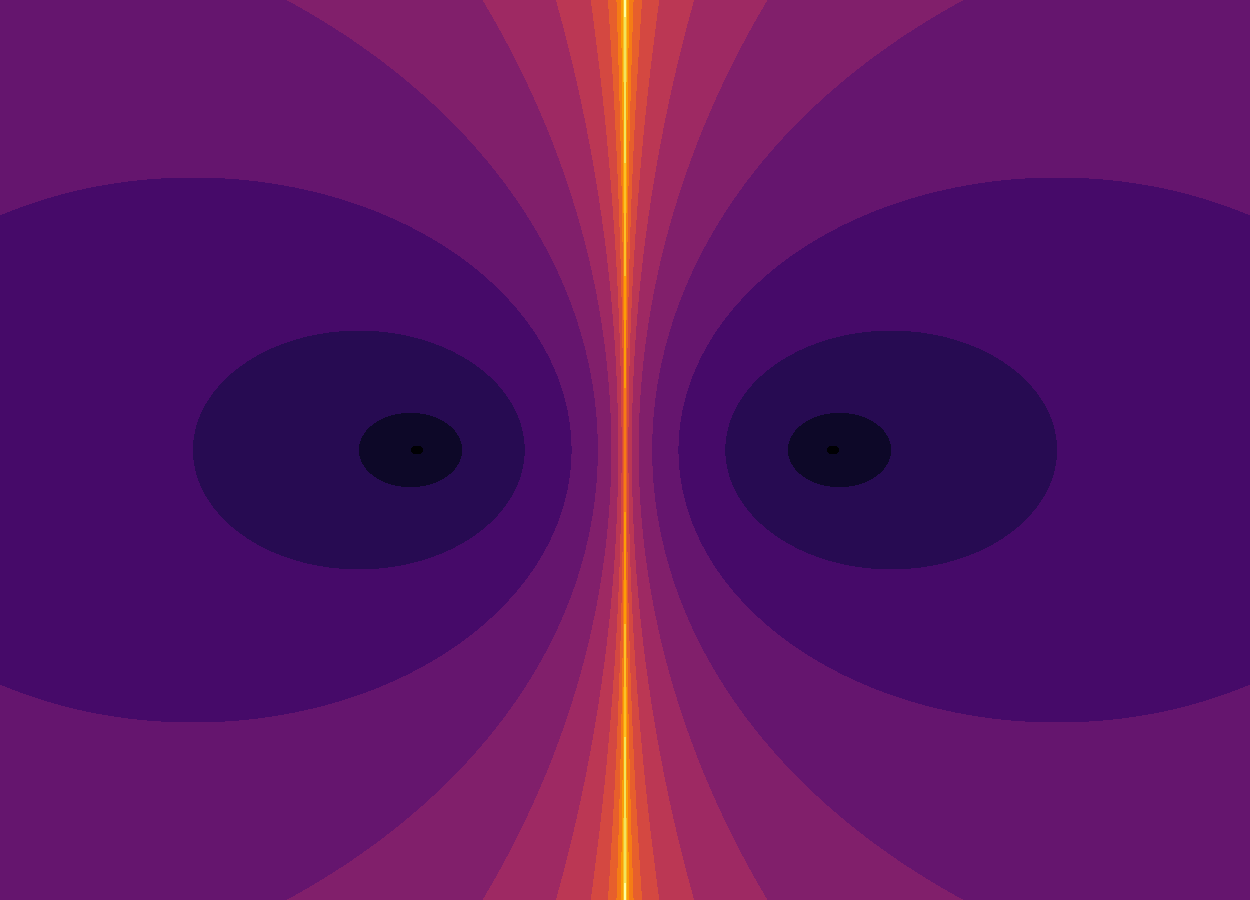
\includegraphics[scale=0.26]{images/eq1-2.png}
    \caption{Rapidez de convergencia de los puntos de $x^2-1$}
    \label{fig:eq_cuadratica_2}
\end{figure}


Donde podemos ver que al aproximarnos a 0, los ritmos de convergencia tienden a aumentar de manera drástica, al punto de no converger.
Esto se debe a que si evaluamos un valor de $p_n = 0$, $g'(0) = 2x = 2(0) = 0$, indefiniendo el resultado del método en ese punto

Veamos otro ejemplo con un comportamiento curioso, el cual también tiene puntos donde el método se indefine
Sea $f(x) = x^3-x$, que al resolver algebraicamente obtenemos $(x-1)(x-0)(x+1)$ con raices en 1,0,-1.
A partir de su gráfica vemos que existen dos puntos críticos, que determinándolos a través de $f'(x) = 0$ da como resultado $-\frac{1}{\sqrt{3}}, \frac{1}{\sqrt{3}}$. 

\begin{figure}[h]
    \begin{tikzpicture}
\begin{axis}[
axis x line = middle,
axis y line =  center,
grid = minor
]
\addplot[
color=red,
]{x^3-x};
\addplot[only marks] table {
1   0
-1  0
0   0
};
\end{axis}
\end{tikzpicture}
\centering
    \caption{Gráfica de $x^3-x$}
    \label{fig:graph_cubica}
\end{figure}


De esto podemos concluir que $(-\infty,-\frac{1}{\sqrt{3}}) \subset  B(-1)$ y $(\frac{1}{\sqrt{3}}, \infty) \subset  B(1)$. Para el caso de $B(0)$, su determinación es un poco más complicada, ya que debemos tomar en cuenta los puntos crítico, los cuales producirán un efecto cíclico, en este caso de período 2, en Newton-Raphson si se les tome como puntos iniciales o cualquier punto inicial que, después de n iteraciones, haga que la tangente de la función sea igual a uno de ellos \cite{wiersma}. 

Partiendo la premisa anterior premisa, tenemos que determinar en que punto $x_0 = x_2$, es decir $x = N(N(x)) = N^2(x)$.  Este proceso se simplifica ya que $f$ es una función impar y entonces $-f(x) = f(-x)$, por lo tanto a través de simetría tenemos que obtendremos $N^2(x)$ si $-x = N(x)$. Para esto calculamos la función en el método

\begin{gather*}
    N(x) = x - \frac{x^3-x}{3x^2-1} \\
    N(x) = \frac{2x^3}{3x^2-1}
\end{gather*}

luego igualamos a -x y resolvemos

\begin{gather*}
    -x = \frac{2x^3}{3x^2-1}\\
    0 = 5x^3-x\\
    x = \pm \frac{1}{\sqrt{5}} \vee x = 0
\end{gather*}

Y de esto podemos concluir que $(-\frac{1}{\sqrt{5}},\frac{1}{\sqrt{5}}) \subset B(0)$
\\
\\
Ahora bien, veamos que pasa entre los valores de $(-\frac{1}{\sqrt{3}},-\frac{1}{\sqrt{5}})$ y $(\frac{1}{\sqrt{5}},\frac{1}{\sqrt{3}})$. Como la función es simétrica, entonces lo que pasa en $(\frac{1}{\sqrt{5}},\frac{1}{\sqrt{3}})$, será igual que en $(-\frac{1}{\sqrt{3}},-\frac{1}{\sqrt{5}})$. En estos dos intervalos se suceden áreas de convergencia hacia $B(1)$ y $B(-1)$, las cuales se ven divididas por valores los cuales luego de n iteraciones caerían en alguno de los puntos críticos de la función, indefiniendo el método.



Veamos por ejemplo un punto un poco a la izquierda de $\frac{1}{\sqrt{3}}$, por ejemplo 0.5773442692, el cual si evaluamos en Newton, nos devolverá $-18518.03739$, un valor que se encuentra dentro de los puntos convergentes hacia -1, hasta que encontremos un valor cuya n iteración sea $-\frac{1}{\sqrt{3}}$ , el cual al igualar ese valor en el método obtenemos 0.465601, por lo tanto $(\frac{1}{\sqrt{3}},0.465601) \subset  B(-1)$.
Si luego probamos con 0.465600, la siguiente iteración devuelve un número positivo muy grande, que cae dentro de $B(1)$. Este comportamiento se mantendrá hasta que hallemos un número cuya n-esima iteración de como resultado $\frac{1}{\sqrt{3}}$ e indefina la función. 

Estos patrones continúan y se alternan entre cada división causada por valores que iteren hacia alguno de los puntos críticos de la función, y podremos determinar cada una de estas divisiones igualando l a función a uno de los puntos previos obtenidos,, esto nos genera unos patrones curiosos, como puede verse en Figura \ref{fig:eq_cubica_1} y \ref{fig:eq_cubica_2}
\begin{figure}[H]

        \centering
        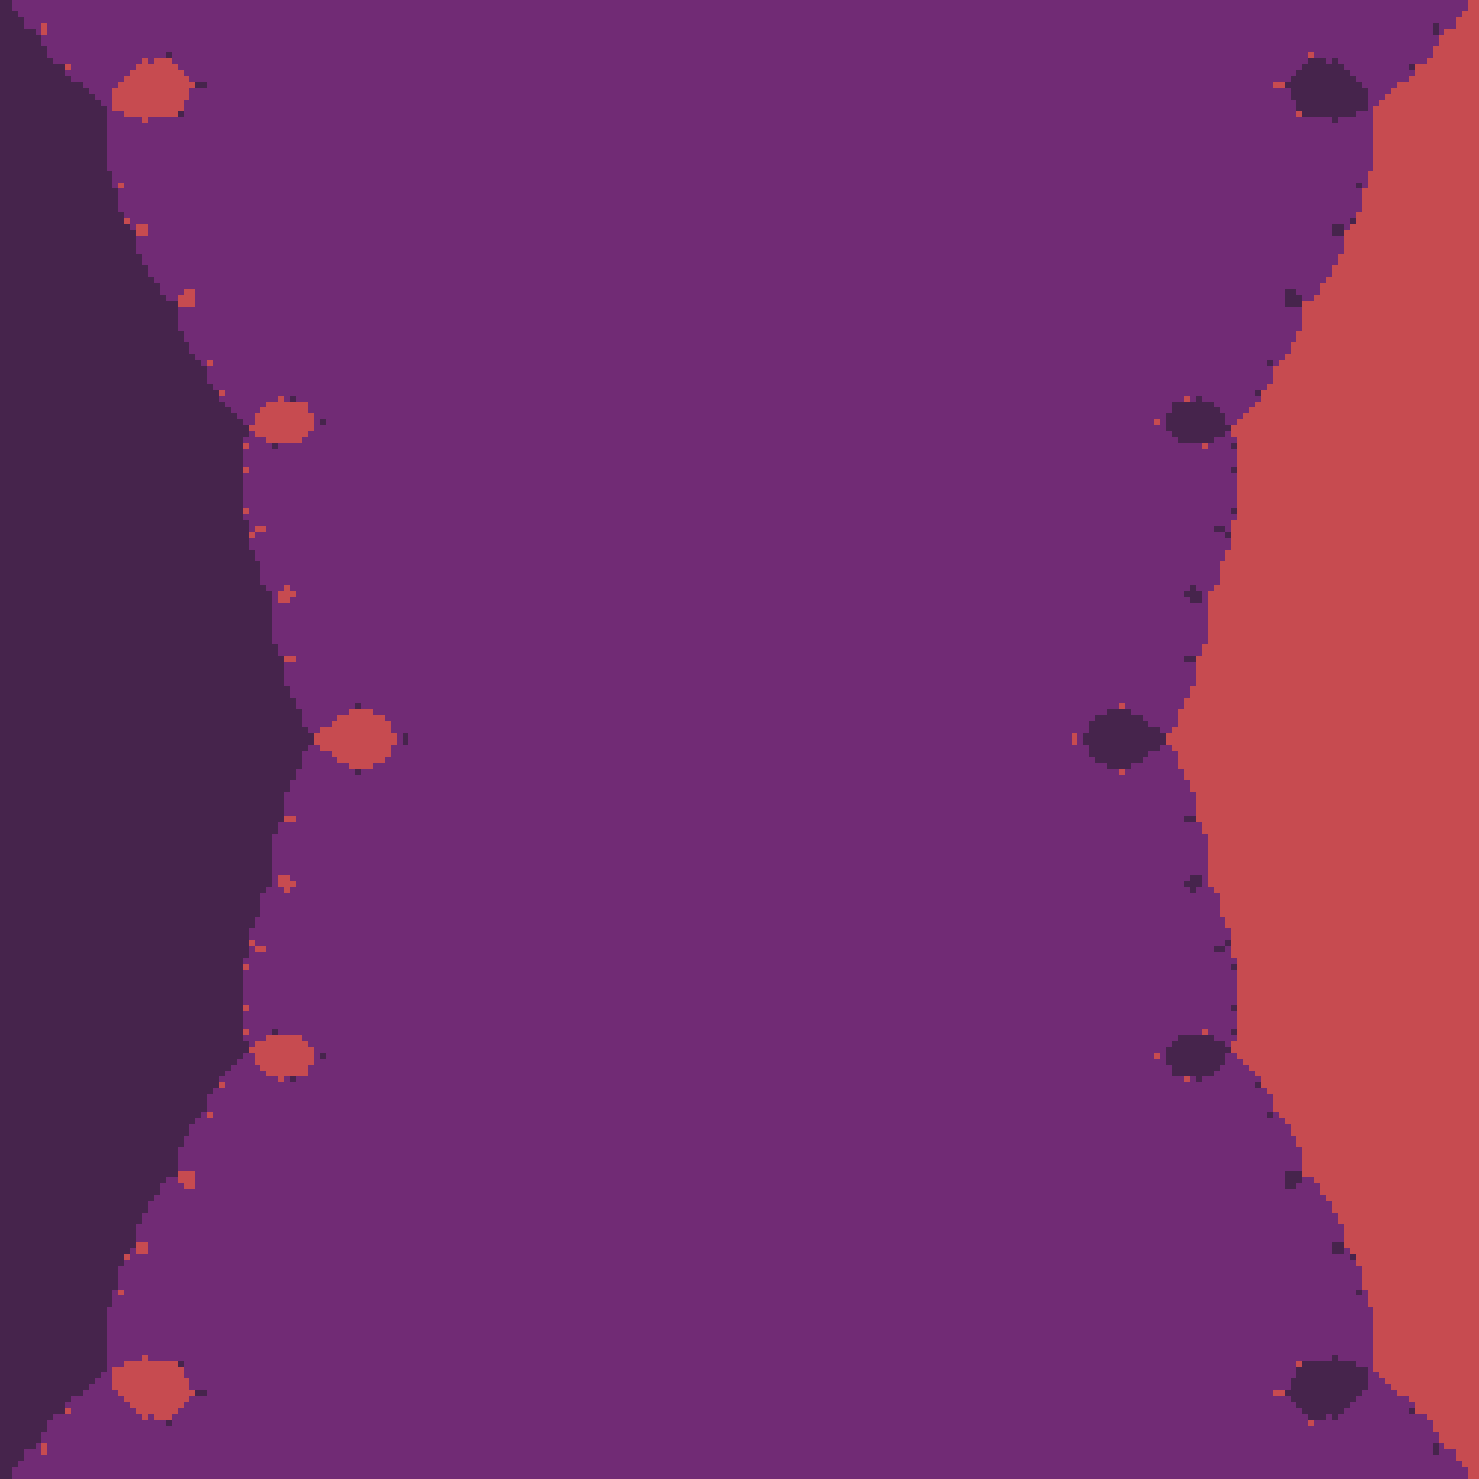
\includegraphics{images/eq2-1.png}
        \caption{Áreas de convergencia de $x^3-x$}
        \label{fig:eq_cubica_1}
\end{figure}
    
\begin{figure}[H]
    \centering
    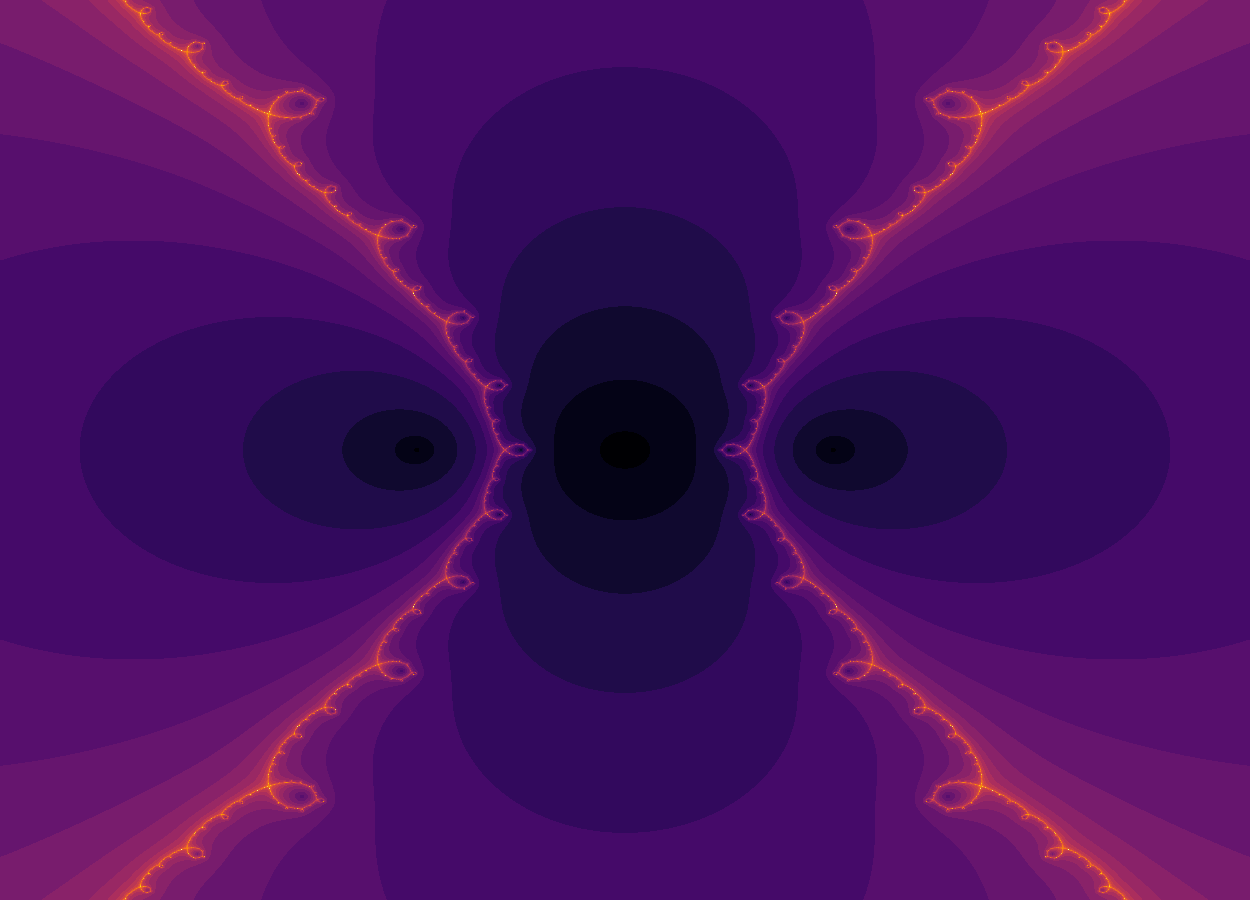
\includegraphics[scale=0.26]{images/eq2-2.png}
    \caption{Rapidez de convergencia de los puntos de $ x^3-x$}
    \label{fig:eq_cubica_2}
\end{figure}

\section{Análisis del error del método de Newton-Raphson}

El error del método de Newton, puede obtenerse a partir de su deducción del método de Taylor, donde 
\begin{displaymath}
p - p_{n+1} =  - (p-p_n)^2 \frac{f''(p)}{2!f'(p)}
\end{displaymath}

es el error obtenido a través de la aproximación polinomial. 
Sin embargo, mediante el Teorema del Valor Medio, puede obtenerse una fórmula más sencilla para obtener el error a lo largo de las iteraciones del método

\begin{displaymath}
f(p_n)= f(p_n) - f(p) = f'(\xi)(p_n-p)
\end{displaymath}
\begin{displaymath}
\frac{f(p_n)}{ f'(\xi)} =(p_n-p)
\end{displaymath}

Donde si $f'(\xi)$ no cambia rápidamente entre p y $p_n$, entonces $f'(\xi) = f'(p)$ y
\begin{displaymath}
(p_n-p)= \frac{f(p_n)}{ f'(\xi)} = p_{n+1} - p_n
\end{displaymath}
obteniendo así la fórmula del error estándar de Newton
\begin{equation}
(p_n-p)=  p_{n+1} - p_n
\end{equation}
\subsection{Análisis sobre la eficiencia del método de Newton-Raphson}

El método de Newton-Raphson, tiene una convergencia cuádratica, como se demostrará partiendo del siguiente teorema

\begin{theorem}
Asumiendo que $f,f',f''  $sean continuas para toda x en las proximidades de $p$ y asumiendo que $f(p) = 0, f'(p) \neq 0 $.Entonces si se escoge lo suficientemente cerca de $p$ , las iteraciones del método de Newton Raphson convergen a $p$. Con un orden de convergencia cuadrático
\end{theorem}

\begin{proof}
Partiendo de 

\begin{displaymath}
\lim_{n->\infty}{\frac{p_{n+1} - p}{p_n - p}} = \lambda
\end{displaymath}
Usaremos el polinomio de Taylor de $f(x)$ en \textit{p}
\begin{displaymath}
 0 = f(p_n) + (p-p_n)f'(p_n) + \frac{(p-p_n)^2}{2}f''(p)
\end{displaymath}
obtenemos
\begin{displaymath}
p - p_{n+1} =  - (p-p_n)^2 \frac{f''(p)}{2f'(p)}
\end{displaymath}
\begin{displaymath}
\frac{|p - p_{n+1}|}{|(p-p_n)^2|} = \frac{f''(p)}{2f'(p)}
\end{displaymath}

\begin{displaymath}
\lim_{n->\infty}{\frac{|p - p_{n+1}|}{|(p-p_n=|)^2}} =  \frac{f''(p)}{2f'(p)}
\end{displaymath}
Lo que prueba que la convergencia del método es cuadrática
\end{proof}


\section{Extensión del método al Dominio de $\mathbb{C}$}

El teorema fundamental del álgebra enuncia lo siguiente:

\begin{theorem}
 Todo polinomio de grado n $n \geq 1$ tiene n raíces complejas
\end{theorem}

Cuya demostración se puede encontrar en \cite{lankham}

A partir de esto, podemos expandir la búsqueda de raíces incluyendo números imaginarios y pasar del plano exclusivamente real, al plano complejo  $\mathbb{C}$ y extender a su vez el método de Newton-Raphson, cuya única modificación será que ahora es capaz de recibir funciones complejas y puntos iniciales del mismo tipo

\begin{equation}
     z = z_{n-1} - \frac{f(z_{n-1})}{f'(z_{n-1})}
\end{equation}

Por ejemplo, sea $f(z) = z^2+1, f'(z) = 2z$, veremos que obtenemos las  raíces $-i,i$ con la siguiente imagen de sus puntos de convergencia
\begin{figure}[H]
    \centering
    
\includegraphics{images/eq3-1.png}
    \caption{ Zonas de convergencia de $ x^2+1$}
    \label{fig:eq_cuad_compleja_1}
\end{figure}

y si colocamos el mapa de la rapidez de convergencia de sus puntos (Los colores más claros indican mayor cantidad de iteraciones)
\begin{figure}[H]
    \centering
    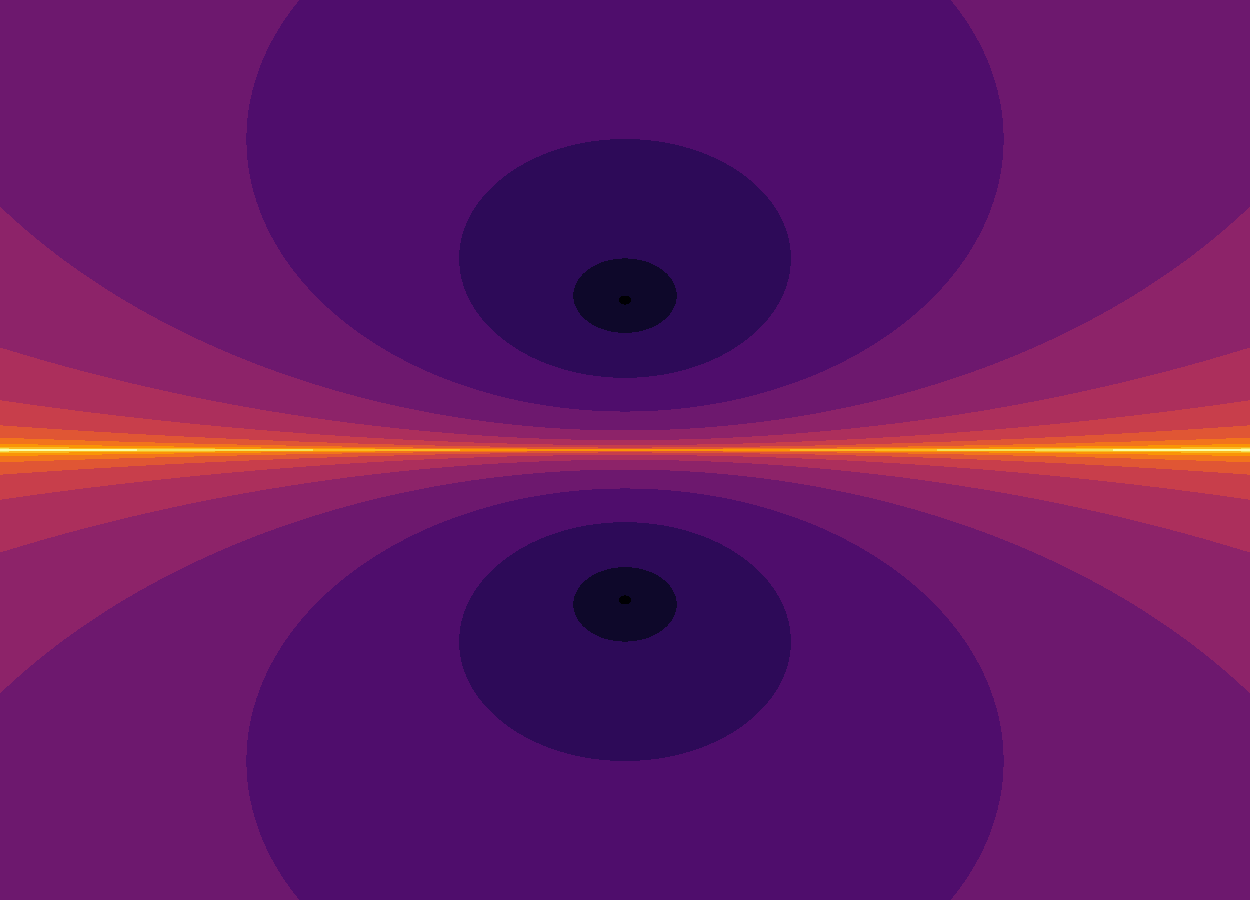
\includegraphics[scale=0.26]{images/eq3-2.png}
    \caption{Rapidez de convergencia de los puntos de $ x^2+1$}
    \label{fig:eq_cuad_compleja_2}
\end{figure}
Comportándose muy similar a la función vista previamente en Figura \ref{fig:eq_cuadratica_2}, con la división siendo en este caso el eje de los reales 

Pero que pasa con funciones de grado $n \geq 2$
Si observamos la función $f(z) = z^3-1$, obtenemos las raíces $(-0.5,-0.866i),(-0.5+0.866i),(1+0i)$ y al generar su mapa de convergencia, obtenemos la siguiente imagen, la cual genera un patrón interesante
\begin{figure}[H]
    \centering
    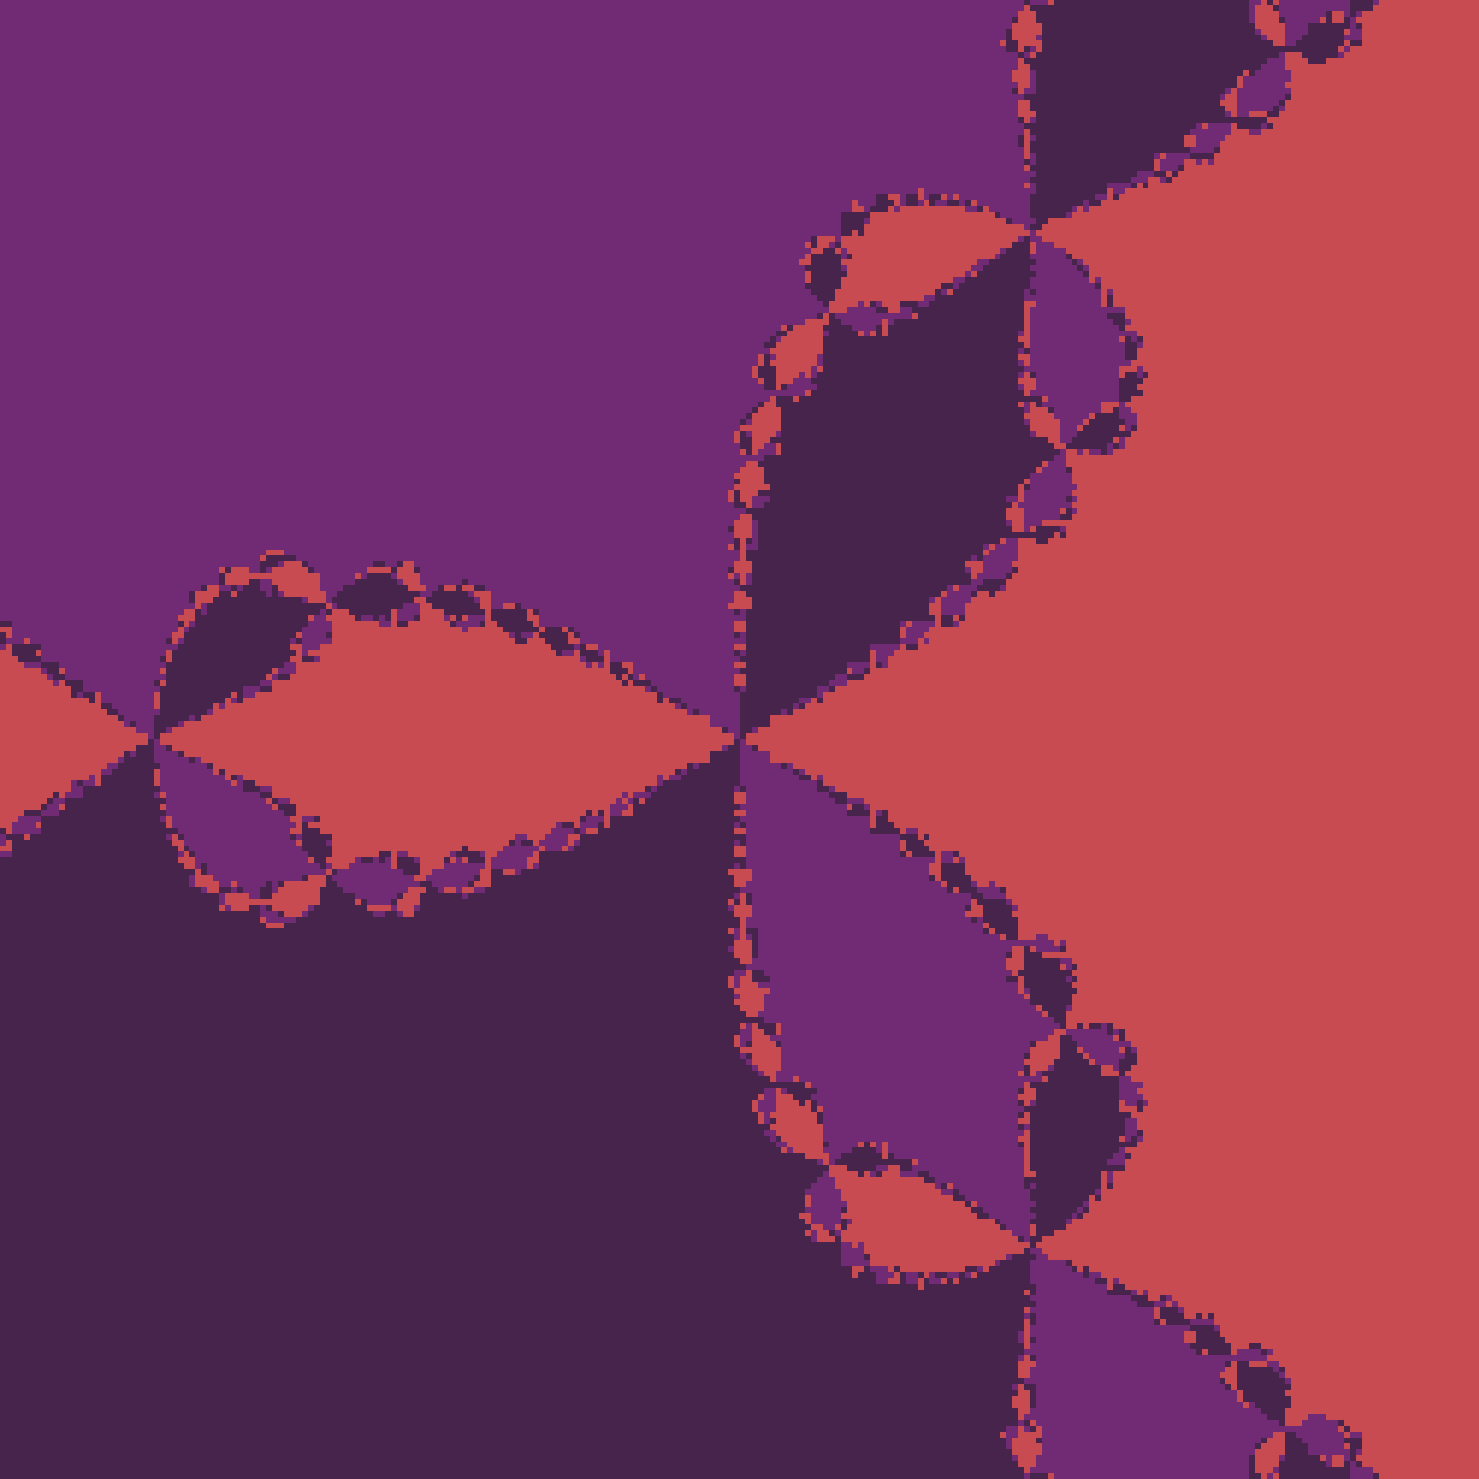
\includegraphics{images/eq4-1.png}
    \caption{Zonas de convergencia de los puntos de $ x^3-1$}
    \label{fig:eq_cub_compleja_1}
\end{figure}
y si se gráfica de la rapidez de convergencia de sus puntos vemos lo siguiente
\begin{figure}[H]
    \centering
    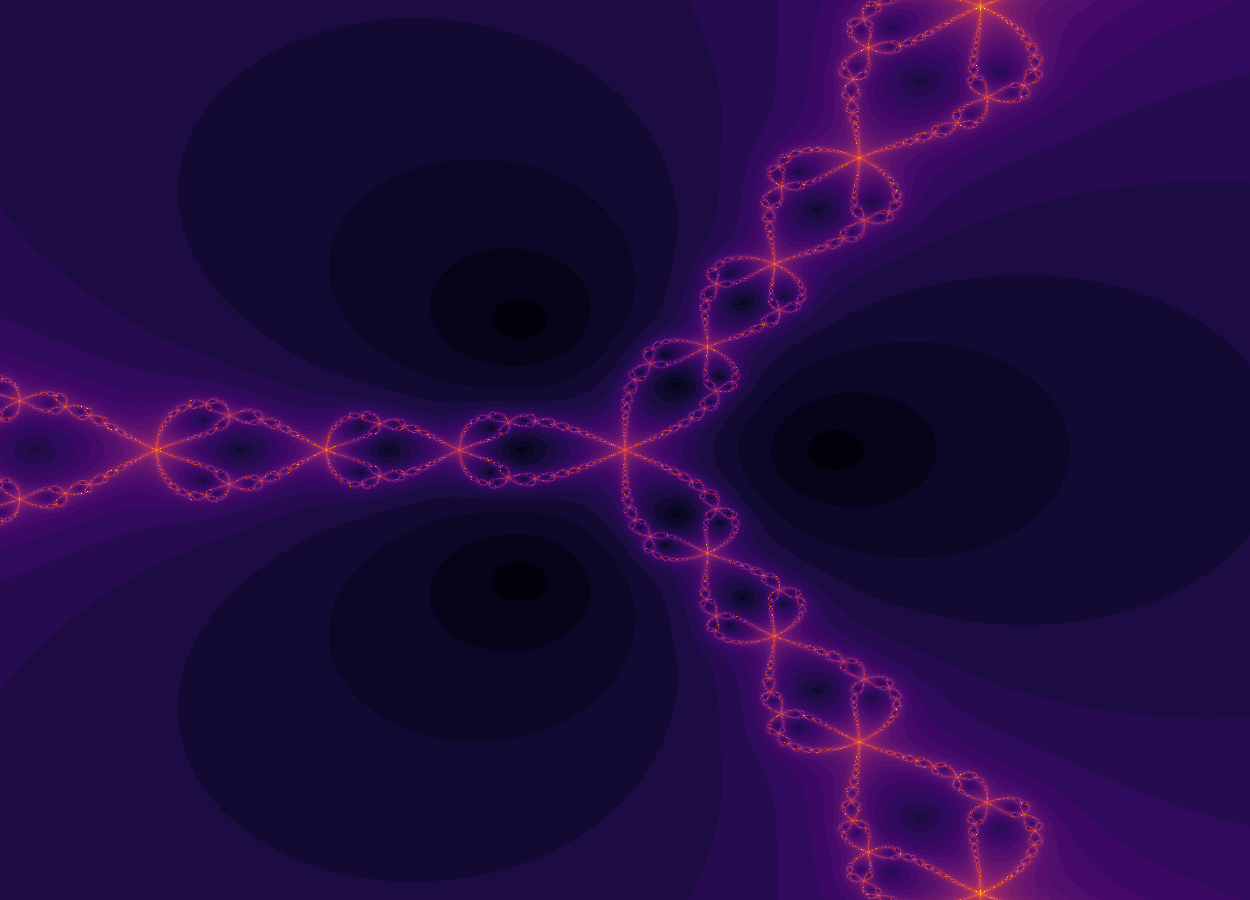
\includegraphics[scale=0.26]{images/eq4-2.png}
    \caption{Rapidez de convergencia de los puntos de $ x^3-1$}
    \label{fig:eq_cub_compleja_2}
\end{figure}
Aquí notamos dos comportamientos inusuales
El primero de ellos es que se forma un fractal muy similar a un conjunto de Julia\cite{badger}, y que se empezaba a vislumbrar en la Figura \ref{fig:eq_cuadratica_2}, donde cerca de los bordes donde comenzaría la siguiente región de otra raíz, observamos una formación que, sin importar el nivel de acercamiento que se le de, contiene colores correspondientes a otras zonas de atracción, los cuales a su vez contienen más de estas zonas de atracción de las demás raíces. Estos fractales son conocidos como fractales de Newton \cite{3b1b}

Podemos ver en esto que se réplica la idea de que entre regiones donde el método tomaría muchas iteraciones o donde fallase, se ven contenidas zonas de atracción hacia las demás raíces, pero además podemos observar que cada zona es dividida entre lugares donde todos los puntos convergen hacia una única raíz o lugares donde se contienen n colores divididos de manera recursiva en estas dos zonas

Además se puede apreciar, como ya se mencionaba, que existen zonas, cerca de los bordes y de los puntos críticos, donde los valores de puntos iniciales tomados de dicho sitio tomarán una gran cantidad de iteraciones en converger, como puede verse en \ref{fig:eq_cubica_1}, extendiendo el comportamiento visto dentro de los reales con al función $x^3-x$.

Dichos comportamientos pueden verse en funciones de mayor grado, como puede verse en los ejemplos ilustrados de la sección correspondiente
\section{Ventajas y desventajas del método }

\subsection{Ventajas}

\begin{itemize}
    \item Tiene una rápida convergencia al ser cuadrático
    \item Requiere pocas iteraciones para obtener una alta precisión en el valor de la aproximación
    \item Requiere únicamente un punto inicial
    \item El método es muy fácil de implementar si se cumplen las condiciones que le validan
\end{itemize}

\subsection{Desventajas}

\begin{itemize}
    \item La aproximación inicial debe de estar lo bastante cercana a \textit{p} como para que se cumpla la  condición de que $( p - p_o )^2$ es descartable, caso contrario el método de Newton puede nunca converger independientemente del número de iteraciones \cite{burden}
    \item $f'$ debe de ser continua y debe de conocerse, de lo contrario el método no puede ser aplicado
    \item Si existe algún máximo o mínimo dentro del intervalo de interés, el método no converge
\end{itemize}
\section{Pseudocódigo}
\begin{algorithm}
\SetKwComment{Comment}{/* }{ */}

\caption{Método de Newton-Raphson en $\mathbb{C}$ }
\KwIn{aproximación inicial $z_0$, tolerancia TOL, máximo número de iteraciones $n_{max}$}\
\KwOut{solución aproximada a  \textit{p} o mensaje de error}
$ i = 1$ 
\BlankLine
$z = z_0 - f(z_0)/f'(z_0)$
\BlankLine
\While{$i \le n_max $}{
    \If{$\|z-z_0\|<TOL$}{\tcp{Procedimiento exitoso}\Return{z}} 
    $i = i + 1$
    \BlankLine
    $z = z_0$
}
\Return \KwOut{"El metodo fallo luego de N iteraciones, N="$n_{max}$}
\end{algorithm}

\section{Ejemplos} 
Encuentre  las raíces de los siguientes polinomios utilizando Newton-Rahpson y muestre el gradiente de convergencia de la función:


\textbf{Función:}$x^7-x-1$

\textbf{Raíces:}

\begin{center}
\begin{tabular}{ c c }
 (-0.8099-0.2629i) & (-0.8099+0.2629i) \\
 (-0.3636-0.9526i) & (-0.3636+0.9526i) \\
 (0.6171-0.9009i) & (0.6171-0.9009i) \\  
 (1.1128-0i)  
\end{tabular}
\end{center}


\begin{figure}[H]
    \centering
    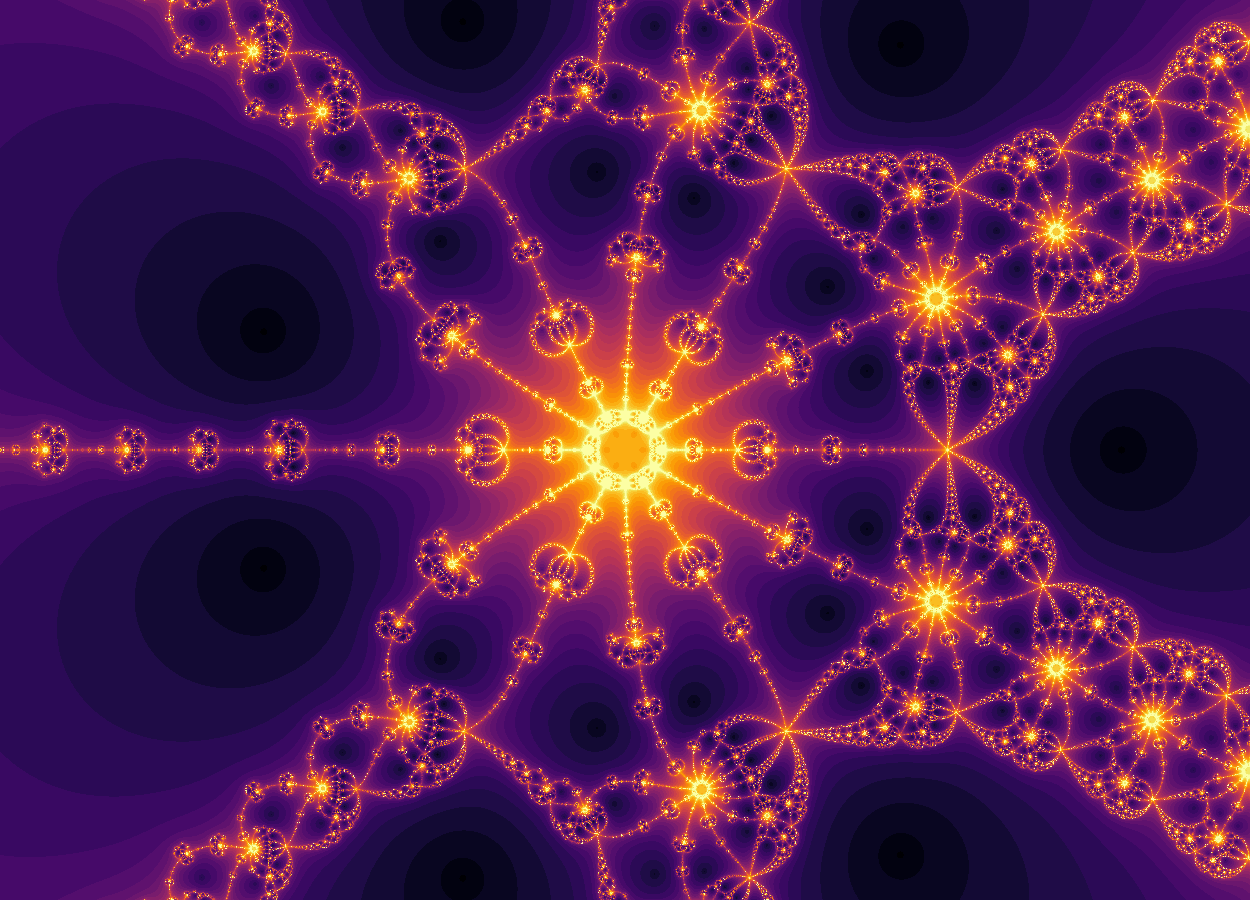
\includegraphics[scale=0.26]{images/ej1.png}
    \caption{Fractal generado por $x^7-x-1$}
    \label{fig:ej_1}
\end{figure}

\textbf{Función:}$x^6-x^3+11$

\textbf{Raíces:}

\begin{center}
\begin{tabular}{ c c }
 (-1.2523-0.8098i) & (-1.2523+0.8098i) \\
 (-0.0752-1.4894i) & (-0.0752+1.4894i) \\
 (1.3275-0.6796i) & (1.3275+0.6796i)
\end{tabular}
\end{center}

\begin{figure}[H]
    \centering
    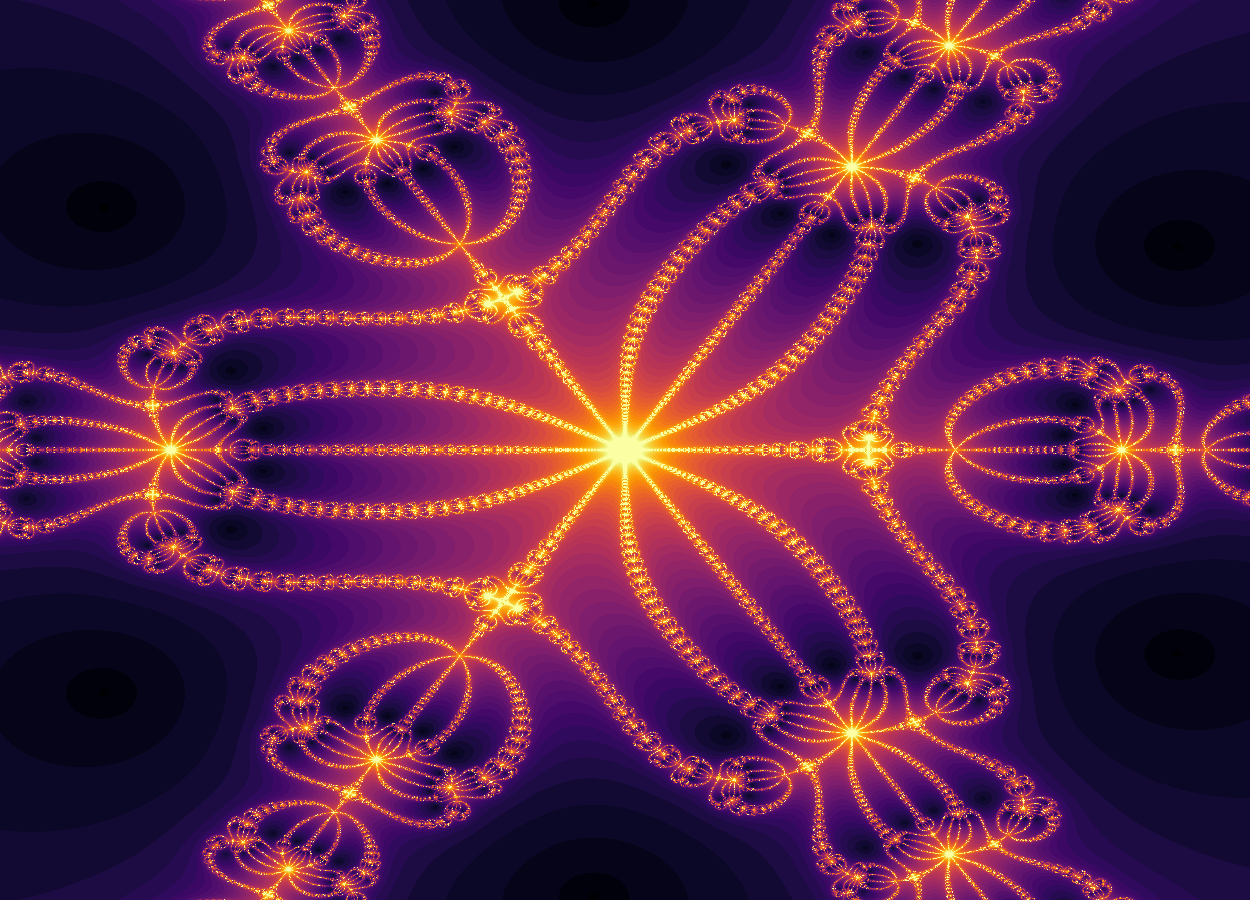
\includegraphics[scale=0.26]{images/ej2.png}
    \caption{Fractal generado por $x^6-x^3+11$}
    \label{fig:ej_2}
\end{figure}

\textbf{Función:}$x^4-x^2-1$

\textbf{Raíces:}

\begin{center}
\begin{tabular}{ c c  }
 (-1.272+0i) & (-0-0.7862i) \\
 0.7862i & (1.272+0i)
\end{tabular}
\end{center}

\begin{figure}[H]
    \centering
    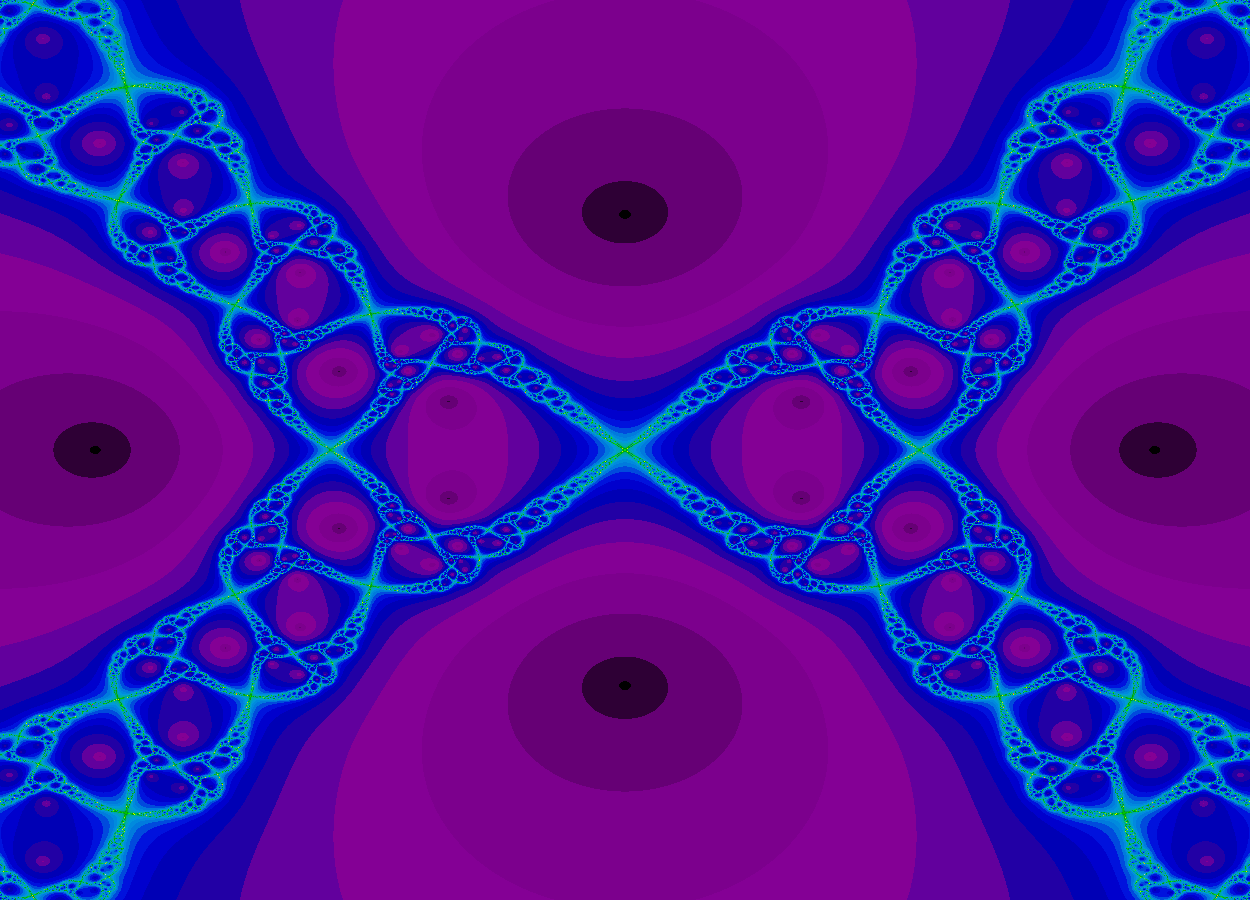
\includegraphics[scale=0.26]{images/ej3.png}
    \caption{Fractal generado por $x^4-x^2-1$}
    \label{fig:ej_3}
\end{figure}

\textbf{Función:}$x^6-3x^2-2x$

\textbf{Raíces:}

\begin{center}
\begin{tabular}{ c c  }
    (-1+0i) & (-0.7413+0i) \\ 
    0i & (0.1472-1.3576i) \\ 
    (0.1472+1.3576i) & (1.4469+0i)
 
\end{tabular}
\end{center}

\begin{figure}[H]
    \centering
    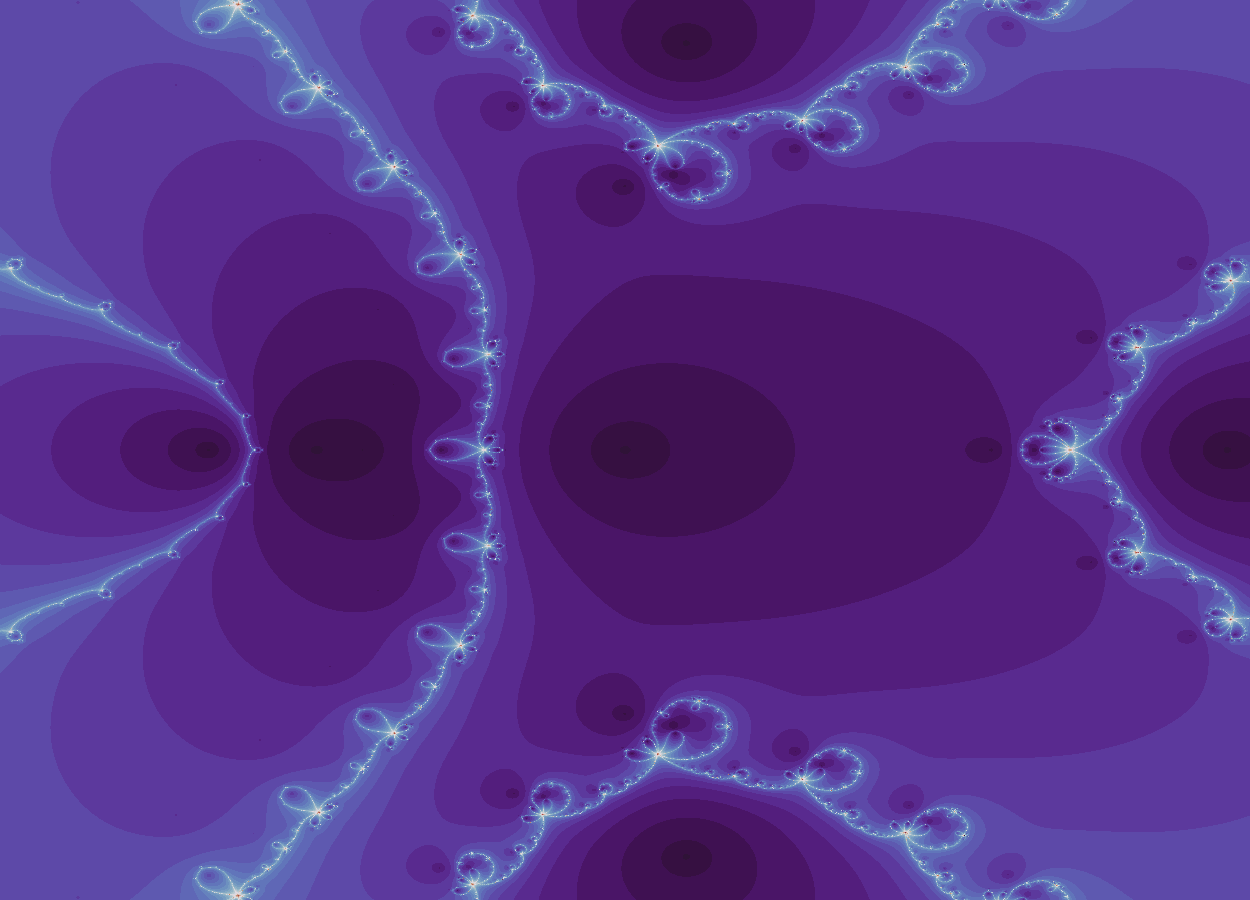
\includegraphics[scale=0.26]{images/ej4.png}
    \caption{Fractal generado por $x^6-3x^2-2x$}
    \label{fig:ej_4}
\end{figure}

\textbf{Función:}$x^7-x^2+1$

\textbf{Raíces:}

\begin{center}
\begin{tabular}{ c c  }
 (-0.8398+0i) & (-0.7555-0.7411i) \\ 
 (-0.7555+0.7411i) & (0.2945-1.0774i) \\ 
 (0.2945+1.0774i) & (0.8809-0.2758i) \\
 (0.8809+0.2758i)
\end{tabular}
\end{center}

\begin{figure}[H]
    \centering
    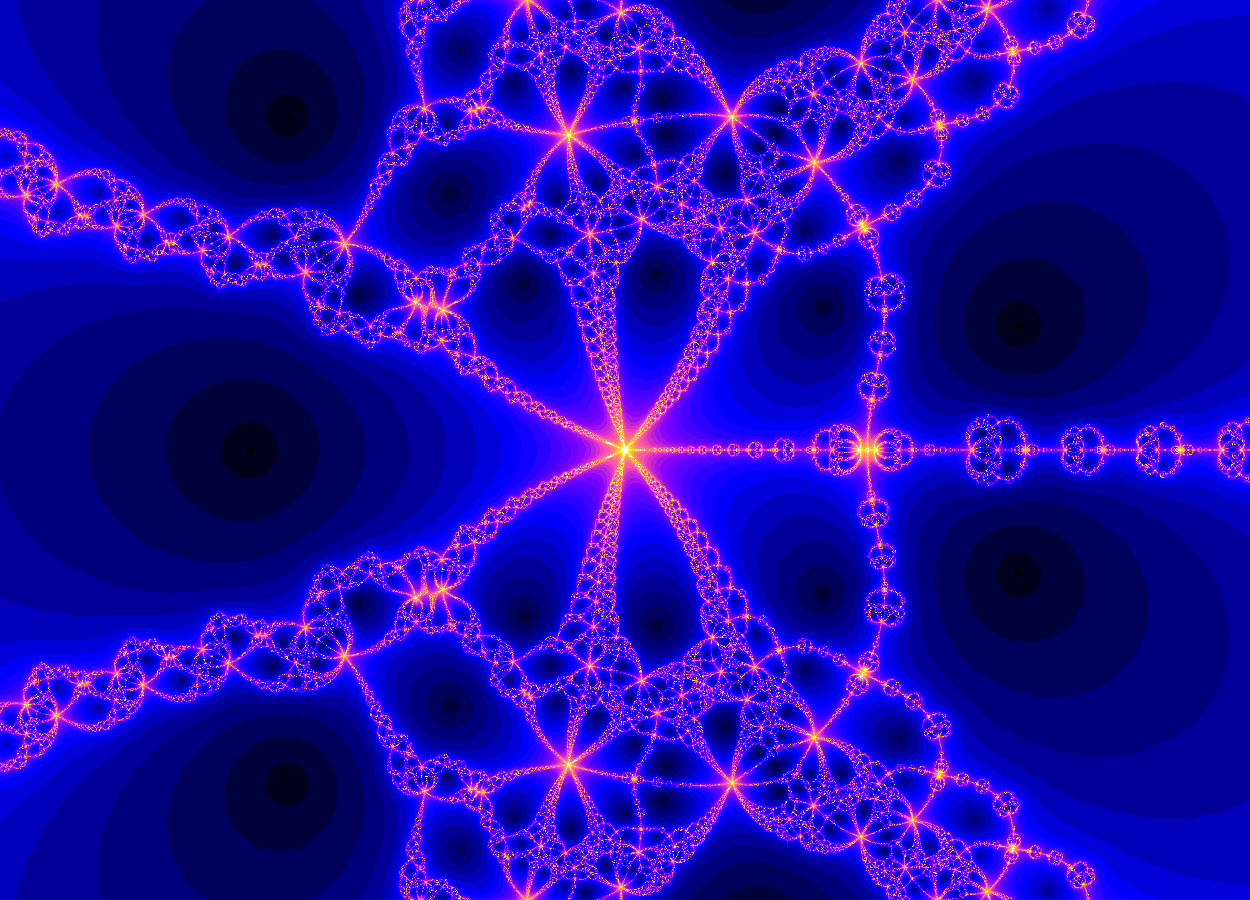
\includegraphics[scale=0.26]{images/ej5.png}
    \caption{Fractal generado por $x^7-x^2+1$}
    \label{fig:ej_5}
\end{figure}

\section{Referencias}



\printbibliography

\end{document}
